\documentclass[fancy, masters,twoside]{byuthesis}
% Class options are simple/fancy and masters/phd.
% Leave options blank for defaults.
% Defaults are simple for document style, and masters for degree type.


%%%%%%%%%%%%%%%%%%%%%%%%%%%%%%%
% Custom options and packages %
%%%%%%%%%%%%%%%%%%%%%%%%%%%%%%%
% Define path to figure files
\graphicspath{{figures/}}

% Define sequences of Latin text to fill space in example documents
% (not needed for your thesis -- delete or comment out if you'd like)
\usepackage{blindtext}


%%%%%%%%%%%%%%%%%%%%%%%%%%%%%%
% Define title page elements %
%%%%%%%%%%%%%%%%%%%%%%%%%%%%%%
% Thesis title for required BYU title page
\title{Evaluating Parameter Uncertainty in Transportation Demand Models}

% On the custom title page, use the same title, but format as you like
\customtitle{Evaluating Parameter Uncertainty in Transportation Demand Models}

% Your name goes here:
\author{Natalie Mae Gray}

% This is the date of graduation
\date{April 2021}

% If your degree is not a PhD or MS, then you can overwrite the degree using
\degree{Master of Science}

% Your department
\department{Department of Civil and Construction Engineering}

% The names of your committee members
\committeechair{Gregory S. Macfarlane}
  \committeemember{Grant G. Schultz}
  \committeemember{Daniel P. Ames}

% Include any keywords you would like for your thesis/dissertation
\keywords{sensitivity analysis, transportation demand model, transportation planning, latin hypercube sampling, monte carlo simulation}


%%%%%%%%%%%%%%%%%%%%%%%%%%%%%%%%%%
% ---Bibliography source file--- %
%%%%%%%%%%%%%%%%%%%%%%%%%%%%%%%%%%


%%%%%%%%%%%%%%%%%%%%%%%%%%%%%%%%%%
% ---Bibliography source file--- %
%%%%%%%%%%%%%%%%%%%%%%%%%%%%%%%%%%
%  Default is references.bib
%
\makepagestyle{myrefs}
\makeevenhead{myrefs}%
    {\normalfont\small\slshape\thepage}{}{\normalfont\small\slshape References}
\makeoddhead{myrefs}%
    {\normalfont\small\slshape References}{}{\normalfont\small\slshape\thepage}
\bibliography{}

\newlength{\cslhangindent}
\setlength{\cslhangindent}{1.5em}
\newlength{\csllabelwidth}
\setlength{\csllabelwidth}{3em}
\newlength{\cslentryspacingunit} % times entry-spacing
\setlength{\cslentryspacingunit}{\parskip}
% for Pandoc 2.8 to 2.10.1
\newenvironment{cslreferences}%
  {}%
  {\par}
% For Pandoc 2.11+
\newenvironment{CSLReferences}[2] % #1 hanging-ident, #2 entry spacing
 {% don't indent paragraphs
  \setlength{\parindent}{0pt}
  % turn on hanging indent if param 1 is 1
  \ifodd #1
  \let\oldpar\par
  \def\par{\hangindent=\cslhangindent\oldpar}
  \fi
  % set entry spacing
  \setlength{\parskip}{#2\cslentryspacingunit}
 }%
 {}
\usepackage{calc}
\newcommand{\CSLBlock}[1]{#1\hfill\break}
\newcommand{\CSLLeftMargin}[1]{\parbox[t]{\csllabelwidth}{#1}}
\newcommand{\CSLRightInline}[1]{\parbox[t]{\linewidth - \csllabelwidth}{#1}\break}
\newcommand{\CSLIndent}[1]{\hspace{\cslhangindent}#1}

\providecommand{\tightlist}{%
  \setlength{\itemsep}{0pt}\setlength{\parskip}{0pt}}

%%%%%%%%%%%%%%%%%%%%%%%%%%
% --- Begin Document --- %
%%%%%%%%%%%%%%%%%%%%%%%%%%
\begin{document}


%%%%%%%%%%%%%%%%%%%%%%%%%%%%%%%%%%%%%%%%%%%%%%%%%%%%%%%
% --- Front matter (probably don't need to change)--- %
%%%%%%%%%%%%%%%%%%%%%%%%%%%%%%%%%%%%%%%%%%%%%%%%%%%%%%%
	\frontmatter

	\titlepage
	\cleardoublepage

	\customtitlepage
	\cleardoublepage


    \begin{abstract}
  \textbf{\emph{NEED}} The abstract of a thesis should describe the
  motivation, objective, overall results, and central findings of the thesis.
  It may have multiple paragraphs if necessary.
  \end{abstract}
  	\cleardoublepage


    \begin{acknowledgments}
  \textbf{\emph{NEED}} Students should acknowledge funding sources. They may also use the
  acknowledgment page to express appreciation for the committee members, friends
  or family who provided assistance in research, writing or technical aspects of
  the dissertation, thesis or selected project. Acknowledgements should be simple
  and in good taste.
  \end{acknowledgments}
  	\cleardoublepage

	\tableofcontents*
	\cleardoublepage

	\listoffigures
	\cleardoublepage

	\listoftables
	\cleardoublepage

	\nomenclature{$c$}{Speed of light in a vacuum inertial frame}
\nomenclature{$h$}{Planck constant}
\nomenclature{$\mathit{Re}$}{Reynolds number}
\nomenclature{$\mathbf{x}$}{State vector}
\nomenclature{$\alpha$}{Angle of attack}
\nomenclature{$\beta$}{Sideslip angle}
\nomenclature{$\gamma$}{Climb angle}
\nomenclature{$p$}{Roll rate}
\nomenclature{$q$}{Pitch rate}
\nomenclature{$r$}{Yaw rate}
\nomenclature{$P$}{Covariance matrix}

\printnomenclature
	\cleardoublepage

%%%%%%%%%%%%%%%%%%%%%
% --- Main Body --- %
%%%%%%%%%%%%%%%%%%%%%
	\mainmatter

\hypertarget{introduction}{%
\chapter{Introduction}\label{introduction}}

\hypertarget{problem-statement}{%
\section{Problem Statement}\label{problem-statement}}

\hypertarget{objectives}{%
\section{Objectives}\label{objectives}}

\hypertarget{literature-review}{%
\chapter{Literature Review}\label{literature-review}}

\hypertarget{overview}{%
\section{Overview}\label{overview}}

Researchers acknowledge that there exists uncertainty in transportation demand models, though few choose to quantify it. This review looks at the types of uncertainty that exists, and research that has been done to evaluate uncertainty. Then, this review considers methods for value sampling, which has been used in research to create a range of input values or parameters.

\hypertarget{types-of-uncertainty}{%
\section{Types of Uncertainty}\label{types-of-uncertainty}}

Uncertainty generally exists from two basic sources: input uncertainty and model uncertainty (Rasouli \& Timmermans, 2012). Input uncertainty includes behavioral and socioeconomic data -- for instance, the number of jobs and residents in a zone might be coded incorrectly -- as well as parameter estimates including automobile operating costs, gasoline costs, and values of time. Model uncertainty can be further divided into specification error and estimation error. Specification error is a failure to estimate the ``true'' model. Estimation error, on the other hand, is a failure to estimate the correct values of model constants and parameters, or taking the mean estimated value as a single parameter.

\hypertarget{input-uncertainty}{%
\subsection{Input Uncertainty}\label{input-uncertainty}}

\hypertarget{model-uncertainty}{%
\subsection{Model Uncertainty}\label{model-uncertainty}}

\hypertarget{sampling-methods}{%
\section{Sampling Methods}\label{sampling-methods}}

There are two popular methods of value sampling, Monte Carlo simulation and Latin hypercube sampling. Monte Carlo simulation draws independently from multiple distributions, while Latin hypercube sampling makes draws that cover the parameter space more efficiently and can capture the joint distribution between two or more parameter values. As a result, Latin hypercube sampling can reduce the number of draws needed to fully re-create the statistical variance in a model, but the amount of reduction is unknown and may not be universal to all problems (Yang et al., 2013).

\hypertarget{summary}{%
\section{Summary}\label{summary}}

In a four-step travel demand model, most error research to this point has focused on input uncertainty, rather than model uncertainty (Rasouli \& Timmermans, 2012). For this study, the estimation error within the model uncertainty is of the most immediate concern.

\hypertarget{model-design-and-methodology}{%
\chapter{Model Design and Methodology}\label{model-design-and-methodology}}

\hypertarget{overview-1}{%
\section{Overview}\label{overview-1}}

\hypertarget{transportation-demand-model}{%
\section{Transportation Demand Model}\label{transportation-demand-model}}

To examine the effects of parameter input sensitivity, we developed a trip-based travel model with four steps:

\begin{enumerate}
\def\labelenumi{\arabic{enumi}.}
\tightlist
\item
  trip generation,
\item
  trip distribution,
\item
  mode choice, and
\item
  destination choice.
\end{enumerate}

Trip generation, the first step, was conducted using socioeconomic (SE) data and household trip productions from Roanoke Valley Transportation Planning Organization \href{https://github.com/xinwangvdot/rvtpo}{RVTPO}. The trip productions were summarized by household sizes, vehicles, and workers, and the weighted mean of each trip purpose was taken. The three trip purposes used are Home Based Work (HBW), Home Based Other (HBO), and Non-Home Based (NHB). Trip attraction was skipped for this analysis.

The second step, trip distribution, used distance and travel time skims from RVTPO. The skims were simplified to use auto, nonmotorized, and transit modes. Travel time for auto used the single occupancy vehicle peak time, nonmotorized travel time used the distance skim multiplied by a factor of average walking speed (3 mph), and transit time used the walk to bus peak time.

Mode choice, the third step, calculates utilities for the three modes. These utilities were exponentiated, added together, and the natural log was taken to get a logsum value for every origin and destination pair. The utility equations for the mode choice model are as follows:

\begin{equation}
\mathrm{drive\_utility} = (\mathrm{coeff\_ivtt}*\mathrm{auto})+(\mathrm{coeff\_cost}*\mathrm{auto\_cost}*\mathrm{DIST})
\label{eq:driveutil}
\end{equation} \begin{equation}
\mathrm{nonmo\_utility} = (\mathrm{k\_nmot}+ 20 * (\mathrm{coeff\_walk1}*\mathrm{nonmotor}))
\label{eq:nonmoutil}
\end{equation} \begin{equation}
\mathrm{trans\_utility} = \mathrm{k\_trn} + (\mathrm{coeff\_ivtt}*\mathrm{transit})
\label{eq:transutil}
\end{equation}

The mode choice parameters (constants and coefficients) were obtained from the \href{https://github.com/byu-transpolab/ustm_resiliency}{USTM Resiliency Model}. These values are shown in Table \ref{tab:MCcoeff} and Table \ref{tab:MCconst}.

\begin{table}

\caption{\label{tab:MCcoeff}Mode Choice Coefficients}
\centering
\begin{tabular}[t]{lrrr}
\toprule
Name & HBW & HBO & NHB\\
\midrule
CIVTT & -0.0450 & -0.0350 & -0.0400\\
CCOST & -0.0016 & -0.0016 & -0.0016\\
CWALK1 & -0.0900 & -0.0700 & -0.0800\\
AUTOCOST & 18.3000 & 18.3000 & 18.3000\\
\bottomrule
\end{tabular}
\end{table}

\begin{table}

\caption{\label{tab:MCconst}Mode Choice Constants}
\centering
\begin{tabular}[t]{lrrr}
\toprule
Name & HBW & HBO & NHB\\
\midrule
K\_TRN & -0.5140 & -0.9853 & -1.3020\\
K\_NMOT & 1.7602 & 0.5448 & -0.5359\\
\bottomrule
\end{tabular}
\end{table}

The final step, destination choice, uses the mode choice logsum as the primary impedance, and a size term calculated using zonal employment. The destination choice utility is the impedance term added to the log of the size term. The destination choice parameters (constants and coefficients) were also obtained from the \href{https://github.com/byu-transpolab/ustm_resiliency}{USTM Resiliency Model}. These values are shown in Table \ref{tab:DCcoeff}.

\begin{table}

\caption{\label{tab:DCcoeff}Destination Choice Parameters}
\centering
\begin{tabular}[t]{lrrr}
\toprule
VAR & HBW & HBO & NHB\\
\midrule
HH & 0.000000 & 1.018700 & 0.2077000\\
I(OTH\_EMP + OFF\_EMP) & 0.000000 & 0.806400 & 0.5626000\\
OFF\_EMP & 0.458600 & 0.403200 & 0.2816000\\
OTH\_EMP & 1.682700 & 0.403200 & 0.2816000\\
RET\_EMP & 0.608700 & 3.813800 & 5.1189000\\
\addlinespace
DISTCAP & 70.000000 & 40.000000 & 40.0000000\\
CLSUM & 1.000000 & 1.000000 & 1.0000000\\
CDIST & -0.080100 & -0.172800 & -0.1157000\\
CDISTSQ & 0.002600 & 0.003400 & 0.0035000\\
CDISTCUB & -0.000009 & -0.000011 & -0.0000133\\
\bottomrule
\end{tabular}
\end{table}

The four-step model gives data in terms of utilities and probabilities. This can be turned into production and attraction trips, and then a highway assignment can be applied using CUBE.

\hypertarget{parameter-sampling}{%
\section{Parameter Sampling}\label{parameter-sampling}}

With this four-step model, MC and LHS methods were used to determine the possible combinations of parameter variance. To identify a standard deviation for each parameter, a coefficient of variation was used. A set coefficient of variation of 0.10 was used for all six mode choice input parameters, and four of the destination choice parameters (HH, OFF\_EMP, OTH\_EMP, and RET\_EMP). Literature had identified a coefficient of variation of 0.30, but for this analysis that caused an unrealistic value of time, and thus it was changed to be 0.10 (Zhao \& Kockelman, 2002). The standard deviation was equal to 0.10 multiplied by the mean, where the mean values in this situation are the base scenario parameters (as identified in Table \ref{tab:MCcoeff}, Table \ref{tab:MCconst}, and Table \ref{tab:MCconst}).

The MC random sampling uses the R function of \texttt{rnorm}. LHS uses the \texttt{lhs} package in R. Since this package only chooses variables on a zero to one scale, the values given use a function to put the random sampling on the right scale needed for the given parameter. The full code for both methods can be found in a public \href{https://github.com/natmaegray/sensitivity_thesis}{GitHub repository}. 100 and 400 draws of random samples for both methods are generated. With these generated parameters, the mode choice model step was run for every set of input parameters for each purpose. The mean logsum value for each run was determined to compare each continuous draw. This allowed us to see how many iterations of which sampling type would be sufficient to show a full range of possible outcomes.

\hypertarget{summary-1}{%
\section{Summary}\label{summary-1}}

A standard four-step model was created in R to create trips, and evaluate sampling methodologies.

\hypertarget{sensitivity-analysis-results}{%
\chapter{Sensitivity Analysis Results}\label{sensitivity-analysis-results}}

\hypertarget{overview-2}{%
\section{Overview}\label{overview-2}}

\hypertarget{sampling-findings}{%
\section{Sampling Findings}\label{sampling-findings}}

The parameters generated were compared for both sampling methods. Figure \ref{fig:parameter100} shows the distributions for the HBW parameters when using 100 draws, and Figure \ref{fig:parameter400} shows how that changes when using 400 draws. These distributions show that LHS gives normally distributed parameters with fewer draws than MC sampling. At 100 draws LHS shows a nearly perfect normal distribution, where there are some discrepancies for the MC generated parameters. Without looking at the mode choice results, these Figures show that LHS is likely to estimate the full variance of the results with much fewer draws.

\begin{figure}

{\centering 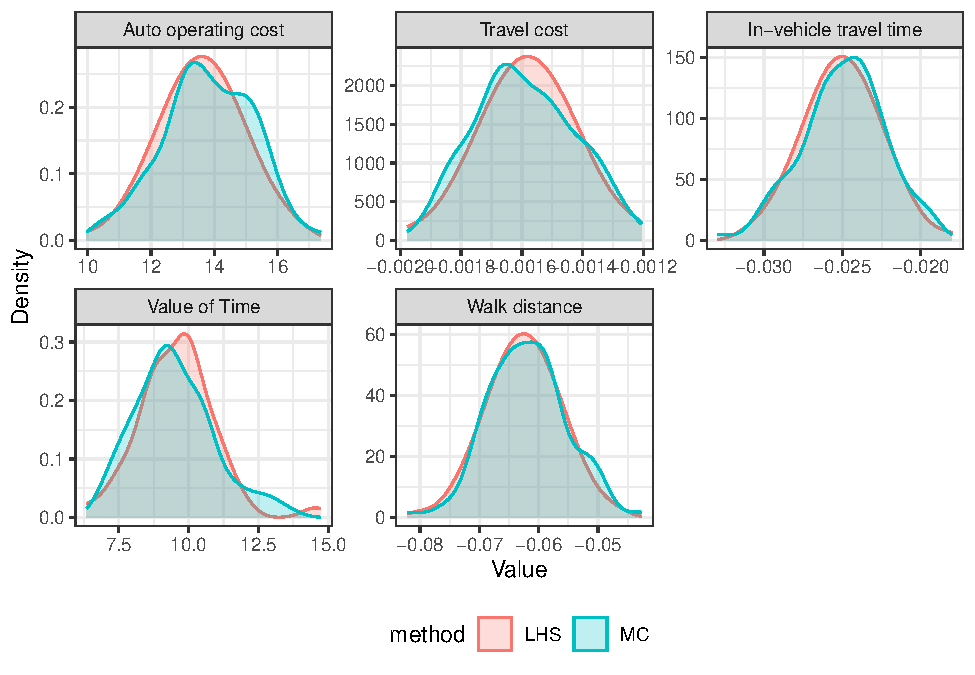
\includegraphics[width=0.75\linewidth]{thesis_files/figure-latex/parameter100-1} 

}

\caption{HBW Distributions for Input Parameters with 100 Draws}\label{fig:parameter100}
\end{figure}

\begin{figure}

{\centering 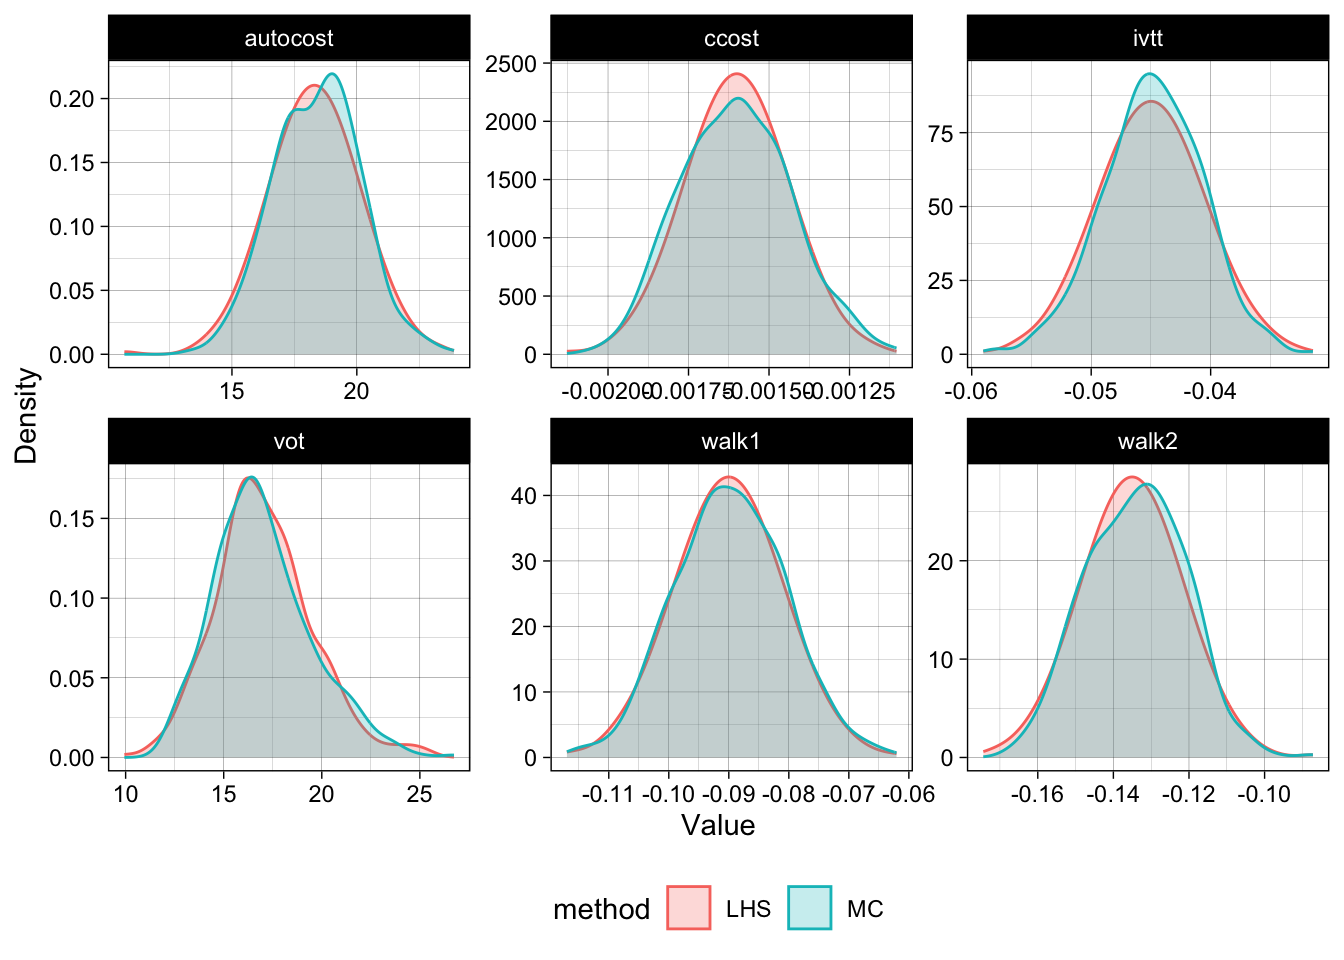
\includegraphics[width=0.75\linewidth]{thesis_files/figure-latex/parameter400-1} 

}

\caption{HBW Distributions for Input Parameters with 400 Draws}\label{fig:parameter400}
\end{figure}

To determine if LHS is effective at a reasonable amount of iterations, the standard deviation was calculated for each additional draw. This value shows how much the mean mode choice logsum value for all zones can vary. When the standard deviation for the draws stabilizes, that shows that the amount of generated parameters has captured all of the possible variances of the results. This can be visualized for each purpose. The HBW results for the cumulative standard deviation are shown in \ref{fig:hbwstats}. The results for the other two purposes (HBO and NHB) are in \ref{fig:hbostats} and \ref{fig:nhbstats} respectively.

\begin{figure}

{\centering 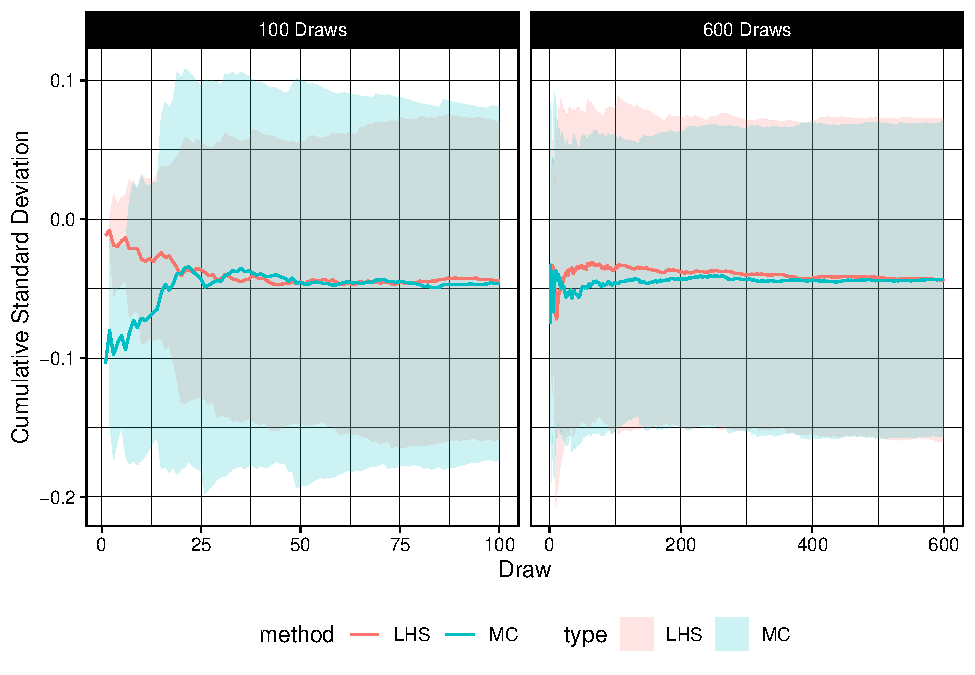
\includegraphics[width=0.75\linewidth]{thesis_files/figure-latex/hbwstats-1} 

}

\caption{HBW Mean Logsum Standard Variation with 100 and 400 Draws}\label{fig:hbwstats}
\end{figure}

\begin{figure}

{\centering 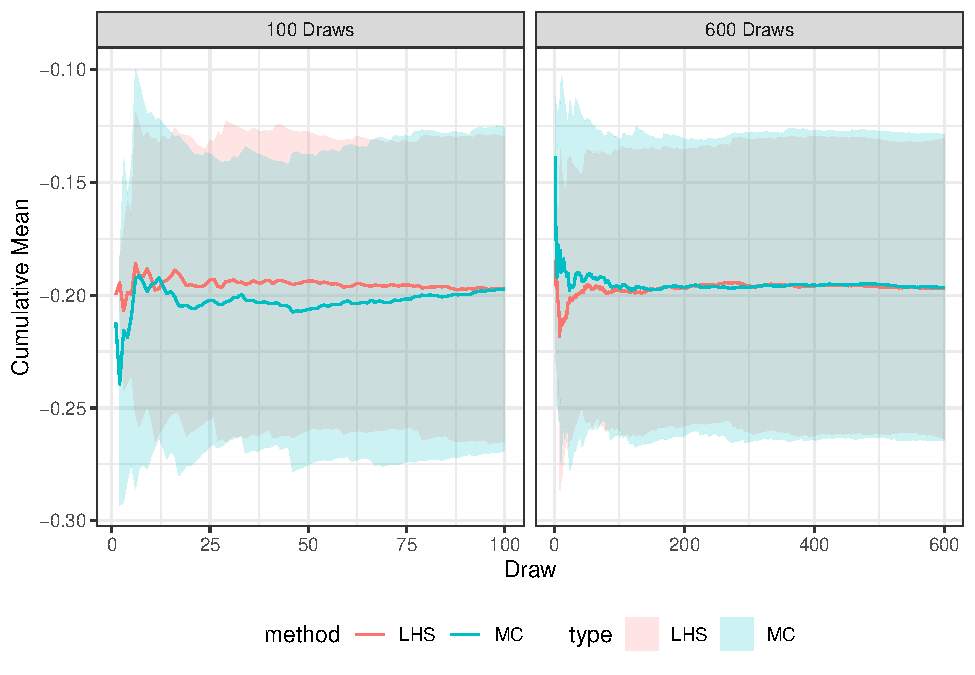
\includegraphics[width=0.75\linewidth]{thesis_files/figure-latex/hbostats-1} 

}

\caption{HBO Mean Logsum Standard Variation with 100 and 400 Draws}\label{fig:hbostats}
\end{figure}

\begin{figure}

{\centering 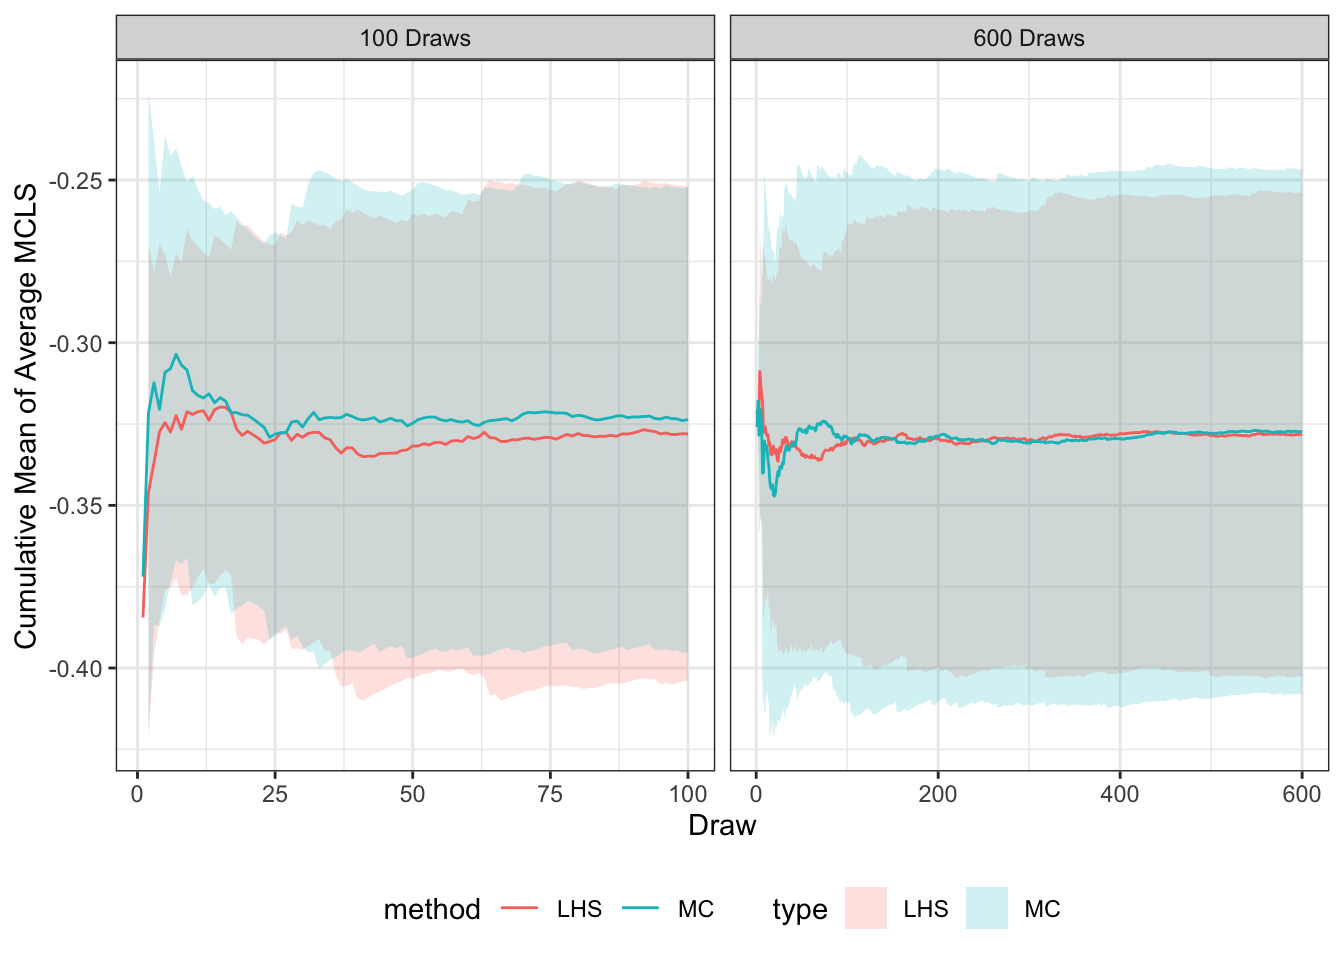
\includegraphics[width=0.75\linewidth]{thesis_files/figure-latex/nhbstats-1} 

}

\caption{NHB Mean Logsum Standard Variation with 100 and 400 Draws}\label{fig:nhbstats}
\end{figure}

For all three trip purposes, the LHS method had its standard deviation stabilized between 100 and 200 draws. The MC method had still not stabilized to the same extent after 400 draws. This shows us that Latin Hypercube Sampling greatly decreases the iterations needed to approximate random sampling methods. Since LHS captures the possible variance at a small enough amount of iterations, it can be used for large transportation demand models.

\hypertarget{roanoke-valley-results}{%
\section{Roanoke Valley Results}\label{roanoke-valley-results}}

A hundred iterations of Latin Hypercube sampling was created with the RVPTO data. Some ways this data can be analyzed to evaluate the range of results is with the highway assignment applied after the four-step model. The coefficient of variation among all iterations for every link in the transportation network can be calculated and compared. Figure \ref{fig:totalvolume} shows, by facility type, how the total volume varies. It can be seen that the higher volume roads, have less variability, and the roads with low volume have more variability.

\begin{figure}

{\centering 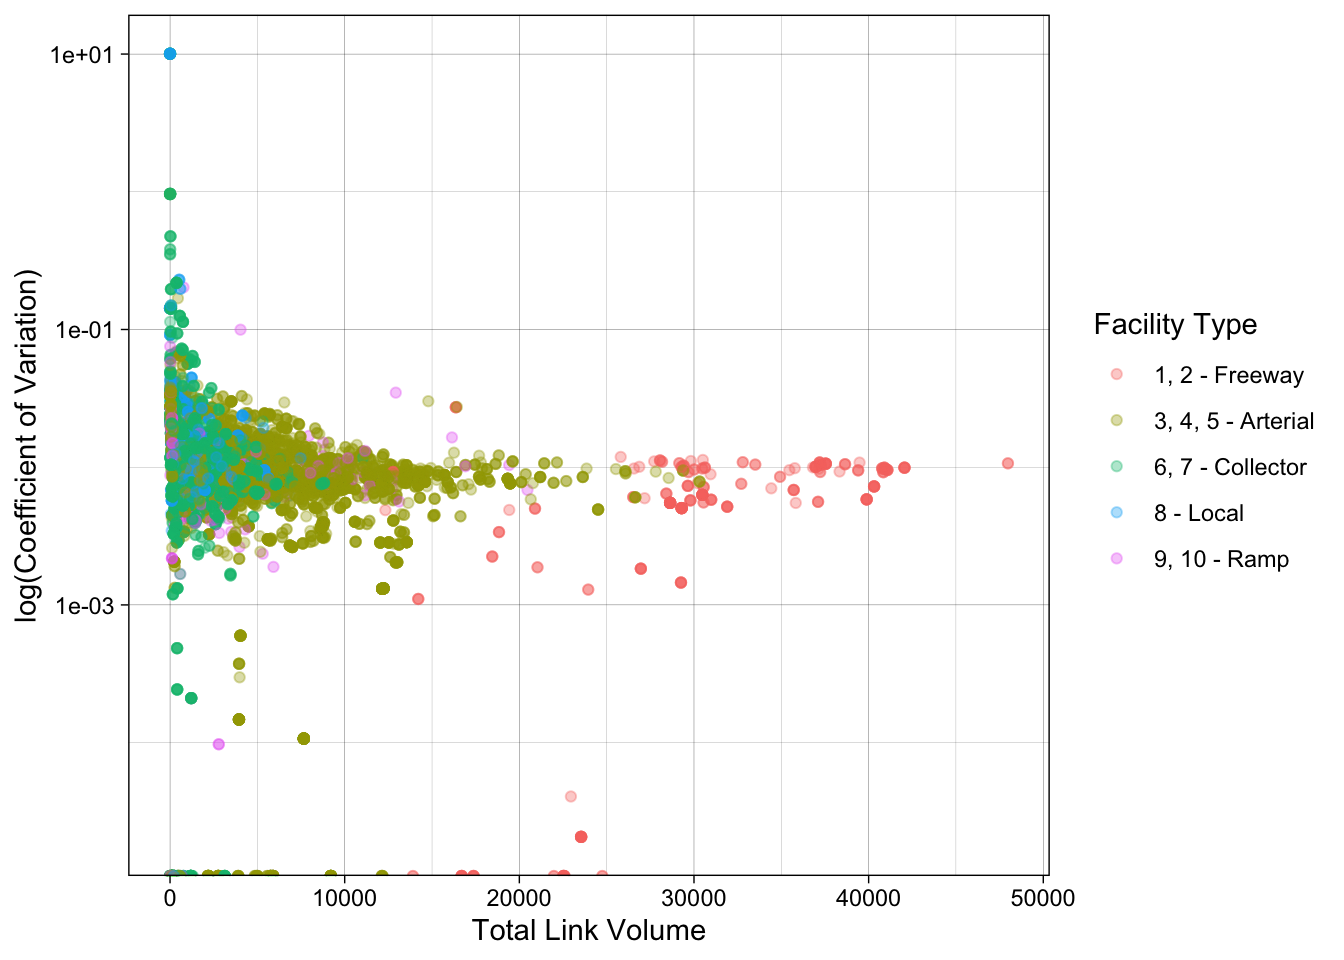
\includegraphics[width=0.75\linewidth]{thesis_files/figure-latex/totalvolume-1} 

}

\caption{Coefficient of Variation of Total Link Volume}\label{fig:totalvolume}
\end{figure}

Variation among a link can also be visualized with a density plot of the total volume across all iterations. In Figure \ref{fig:densityplots} there are three links total volume shown each with different facility types. The green dashed lines are the links measured AAWDT value, and the red dashed lines are the base scenario total volume value. These plots show that across each facility type with an AAWDT value, the variance in total volume is within the range of uncertainty already expected within the model. Since the AAWDT is so different from the Total Volume value, the uncertainty lies more within the model, than within the change in parameter values.

\begin{figure}

{\centering 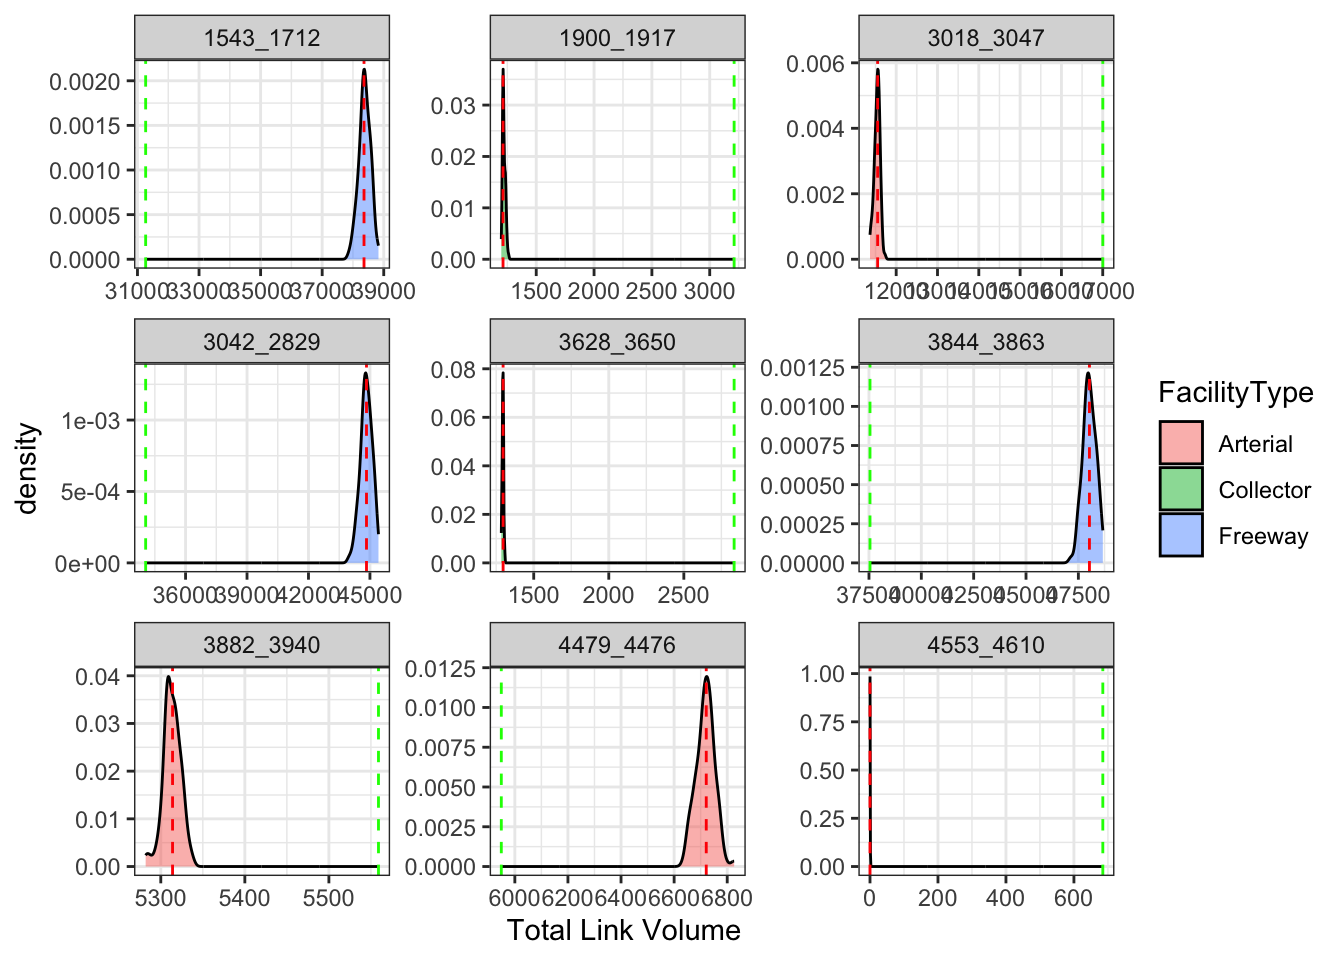
\includegraphics[width=0.75\linewidth]{thesis_files/figure-latex/densityplots-1} 

}

\caption{Total Volume Density for an Individual Link by Facility Type}\label{fig:densityplots}
\end{figure}

Figure \ref{fig:networksd} displays both standard deviation, and the corresponding average volume amoung iterations on each link. This shows that there is a higher standard deviation on roads with high volumes, but a change in 400 vehicles on a road with 40,000 daily volume is minuscule. That is only a 1\% variation in volume which is insignificant.

\begin{figure}

{\centering 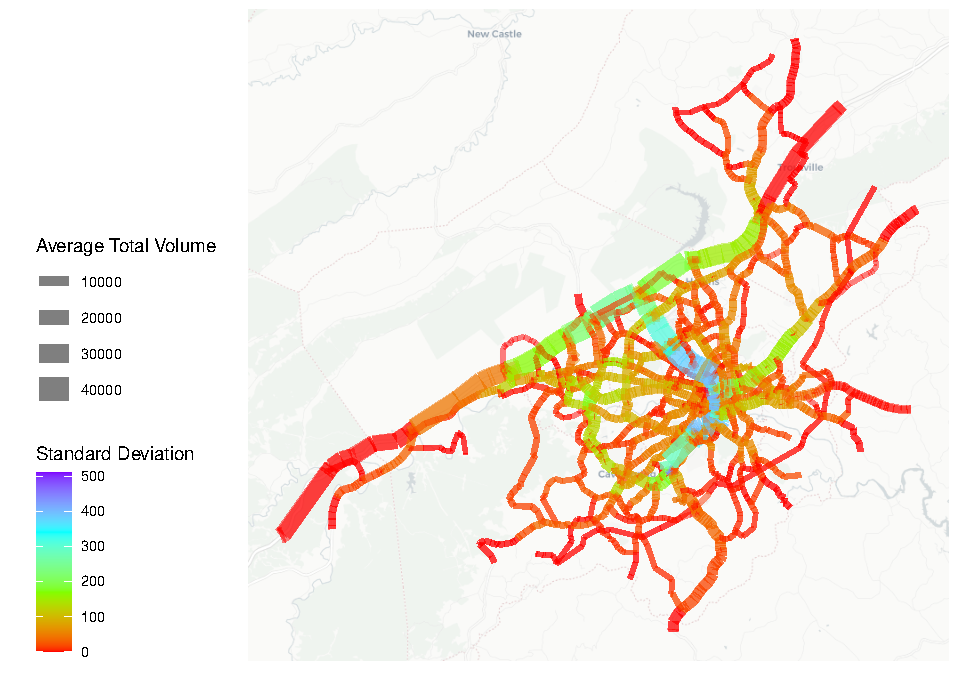
\includegraphics[width=0.75\linewidth]{thesis_files/figure-latex/networksd-1} 

}

\caption{Standard Deviation of Total Volume}\label{fig:networksd}
\end{figure}

Another way to visualize changes among each iteration is to look at how mode choices change. Figure \ref{fig:modechoicetrips} shows that for home based work trips by each origin, the variance among each mode is less than 20\%, and that transit varies the most.

\begin{figure}

{\centering 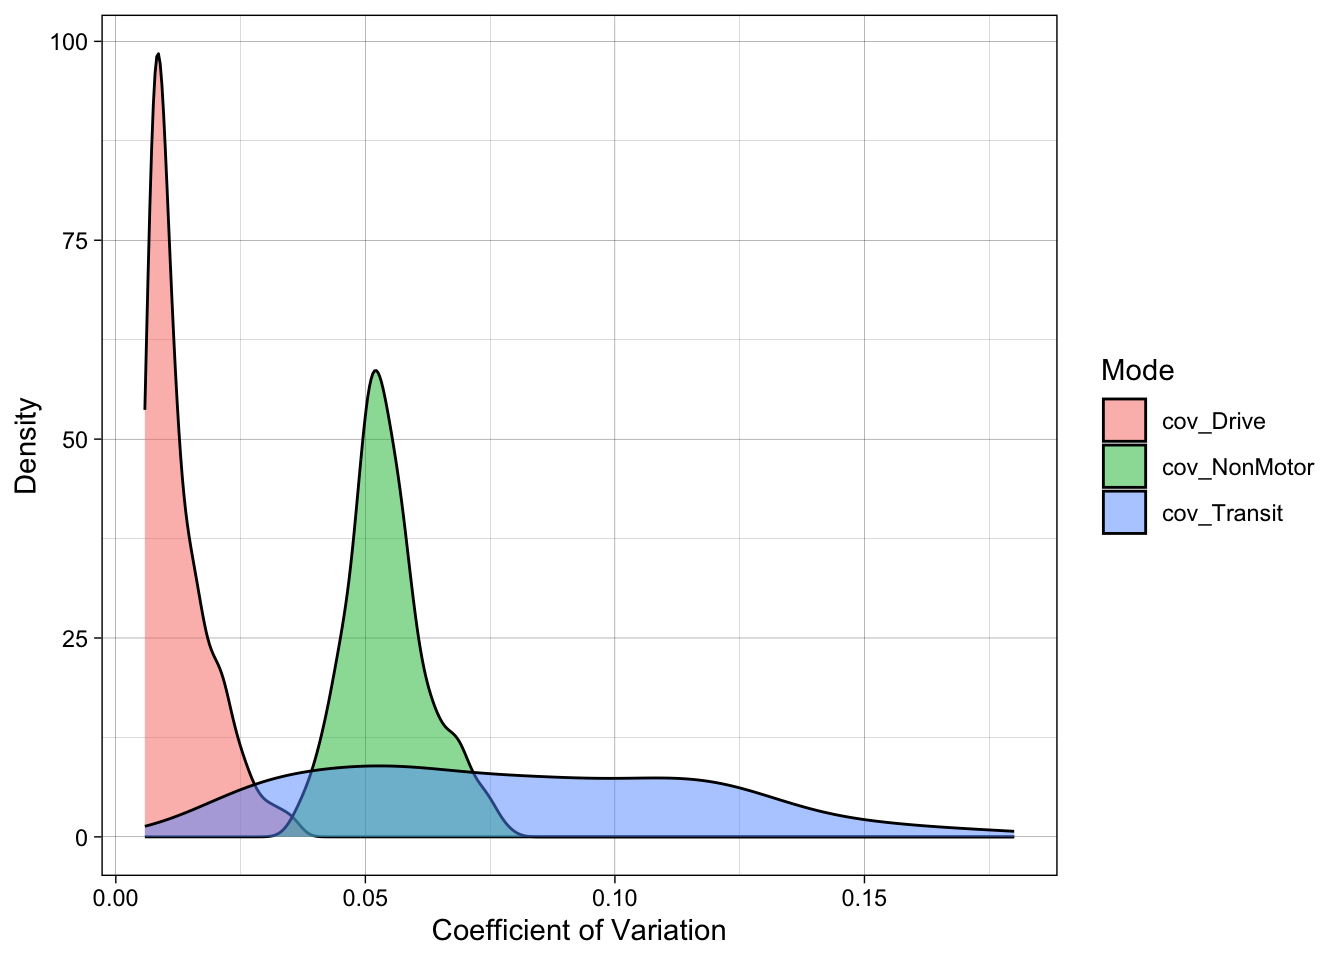
\includegraphics[width=0.75\linewidth]{thesis_files/figure-latex/modechoicetrips-1} 

}

\caption{Origin Desnity for Coefficient of Variation by Mode for HBW Trips}\label{fig:modechoicetrips}
\end{figure}

\hypertarget{summary-2}{%
\section{Summary}\label{summary-2}}

\hypertarget{conclusions}{%
\chapter{Conclusions}\label{conclusions}}

\hypertarget{overview-3}{%
\section{Overview}\label{overview-3}}

\hypertarget{problem-and-objective}{%
\section{Problem and Objective}\label{problem-and-objective}}

\hypertarget{limitations-and-further-research}{%
\section{Limitations and Further Research}\label{limitations-and-further-research}}

\hypertarget{summary-3}{%
\section{Summary}\label{summary-3}}

\hypertarget{references}{%
\chapter*{References}\label{references}}
\addcontentsline{toc}{chapter}{References}

\pagestyle{myrefs}

\hypertarget{refs}{}
\begin{CSLReferences}{1}{0}
\leavevmode\vadjust pre{\hypertarget{ref-rasouli2012uncertainty}{}}%
Rasouli, S., \& Timmermans, H. (2012). Uncertainty in travel demand forecasting models: Literature review and research agenda. \emph{Transportation Letters}, \emph{4}(1), 55--73.

\leavevmode\vadjust pre{\hypertarget{ref-yang2013sensitivity}{}}%
Yang, C., Chen, A., Xu, X., \& Wong, S. (2013). Sensitivity-based uncertainty analysis of a combined travel demand model. \emph{Transportation Research Part B: Methodological}, \emph{57}, 225--244.

\leavevmode\vadjust pre{\hypertarget{ref-zhao2002propagation}{}}%
Zhao, Y., \& Kockelman, K. M. (2002). The propagation of uncertainty through travel demand models: An exploratory analysis. \emph{The Annals of Regional Science}, \emph{36}(1), 145--163.

\end{CSLReferences}

\cleardoublepage
\pagestyle{byu}

%%%%%%%%%%%%%%%%%%%%%%%%
% --- Bibliography --- %
%%%%%%%%%%%%%%%%%%%%%%%%
% printed automatically with CSL
%
%%%%%%%%%%%%%%%%%%%%%
% --- Appendices --- %
%%%%%%%%%%%%%%%%%%%%%


\end{document}
